\chapter{Implémentation}
\section{L'objet Caméra}
\subsection{Description}
L'objet Camera est implémenté dans la classe \textit{Camera.java}.\newline
Celle-ci y regroupe les informations suivante : 
\begin{itemize} 
\item un descriptif de la caméra. Exemple : ``Caméra du Jardin''
\item le protocole de communication à utiliser (http ou rtsp).
\item l'url d'acces. Exemple : ``http://192.168.1.20''
\item le port (par defaut le port 80 est utilisé).
\item le nom d'utilisateur (login).
\item le mot de pass.
\item le canal (necesaire lors de l'utilisation de plusieurs caméras pour une
meme adresse).
\item un identifiant unique appelé \textit{uniqueID} definit par la position de
la caméra dans la liste sur la page d'acceuil.
\item le groupe assigné lors de la mise en route de la détéction de mouvement
(compris entre 0 et 9) appelé \textit{groupeID}.\\
\end{itemize}
Afin de pouvoir communiquer une caméra entre plusieurs \textit{activitées
(activity)} nous avons choisi de rendre cette classe \textit{serializable} pour
ne pas devoir passer une a une chaques caracteristiques.\\
Cette classe contient également une primitive capable de générer un entier
unique pour le couple \textit{uniqueID} et \textit{groupID} afin de pouvoir
lancer plusieurs fenetres de detection de mouvement pour une meme caméra
(\textit{getMotionDetectionID}).
\subsection{Construction de l'objet}
La création d'une caméra se fait via l'interface graphique definit par le
fichier \textit{add\_cam.xml}.\newline
\begin{center}
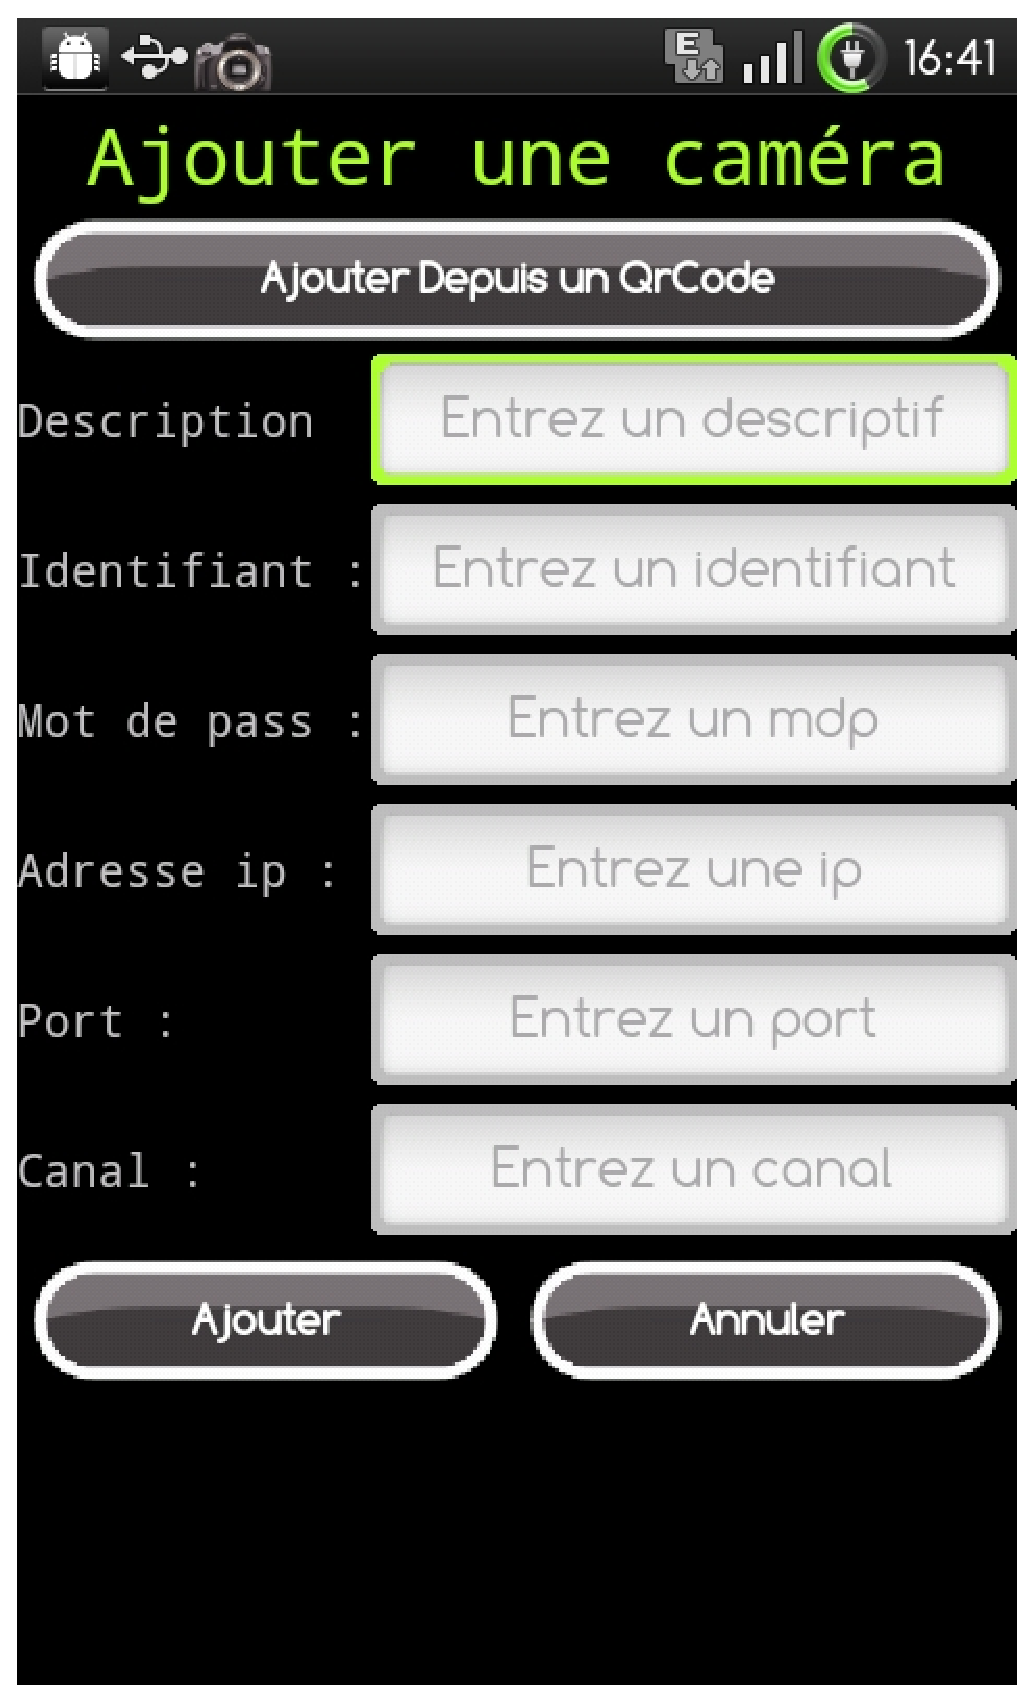
\includegraphics[scale=0.3]{Images/addCamScreenShot.eps}
\newline\end{center} On y retrouve des champs de texte édiatable pour chacunes
des caracteristiques de la caméra ainsi qu'un bouton permettant l'ajout de caméra via
\textit{QrCode}.
\indent Le lecteur de code Qr est implémenté par la bibliothèque
\textit{zxing}\footnote{\label{zxing} http://code.google.com/p/zxing/}. \newline
Lors d'un clic sur ce bouton, nous appelons l'activité 
\textit{SCAN} de la bibliotheque zxing avec comme argument
\textit{QR\_CODE\_MODE}.\newline
Si la bibliothèque n'est pas disponible sur l'appareil, nous faisons appel a
\textit{l'android market} afin de telecharger l'application \textit{zxing} (qui
implémente l'ensemble des fonctions proposées par la bibliothèque).
\newpage
\begin{lstlisting}[caption={Lancement de l'activité zxing ou de l'android
market.}] 
    public void onClick(View v) { try {
            Intent intent = new Intent(
                "com.google.zxing.client.android.SCAN");
            intent.putExtra("SCAN_MODE", "QR_CODE_MODE");
            startActivityForResult(intent, 0);
        } catch (ActivityNotFoundException e) {
            String marketSearch = "market://details?id=com.google.zxing.client.android";
            Intent updateIntent = new Intent(Intent.ACTION_VIEW, Uri.parse(marketSearch));
            startActivity(updateIntent);
        }
    }
\end{lstlisting}

\indent \newline
\indent Lorsque l'activitée \textit{zxing} se termine, l'activité
\textit{addCam} recupere l'adresse de la caméra contenu dans le code Qr puis verrouille les
champs de texte édiatable adresse et port.\\
\indent Pour ajouter la nouvelle
caméra, il ne reste plus  é l'utilisateur qu'é cliquer sur le bouton
\textit{ajouter} pour revenir sur l'écran d'acceuil et constater l'ajout de la caméra. Cependant il reste possible de revenir é l'écran d'acceuil sans sauvegarder les changement en cliquant sur \textit{fermer}.

\subsection{Affichage des Caméras}
Une fois la phase de création reussie, nous avons implémenté une nouvelle
activité permettant d'afficher l'ensemble des caméras ajouter par l'utilisateur.
Cette activité s'appele \textit{Home} et est contenue dans la classe
\textit{Home.java}.\newline
Android defini une cycle de vie pour chaque activitée selon le diagramme
decrit par la \textit{figure 3.1}.
\newline
\indent Ce cycle de vie nous permet d'initialiser, d'interrompre, ou de detruire
les differentes vues et fonctionnalitées de notre activitée. Dans le cas de
l'activité \textit{Home} (qui est l'activité d'acceuil de notre application), ce cycle se traduit par : 
\begin{itemize}
  \item   \underline{onCreate :} \begin{enumerate}
    \item Allouer les ressources a l'aide du construteur de la classe parent
    (\textit{super.onCreate(savedInstanceState});)
    \item Récuperation des préférences de l'utilisateur via un
    \textit{SharedPreferences} décrit utlétieurement.
    \item Démarrage du service de détéction de mouvement.
    \item Affichage d'un pop-up d'aide et astuces (si l'utilisateur n'a pas
    choisi de le desactiver).
    \item Lecture de la liste des caméras deja enregistré si disponible.
    \item Mise a jour et implémentation des \textit{listeners} de la liste
    affichant les caméras.\newline
  \end{enumerate} 
  \item \underline{ onActivityResult :}\newline Lorsqu'un activitée demarre une
  autre activitée via les \textit{startActivity(intent)} ou
  \textit{startActivityForResult(intent, 1)} celle-ci passe en arrière plan pour
  executer l'activité décrite par l'\textit{intent}. Durant cette état elle peut
  être ``tuée'' par le gestionnaire de tache, ou en attente d'un resultat. C'est pourquoi l'état
  onResume de la \textit{figure 3.1} englobe également l'état
  \textit{onActivityResult}.\newline
  Pour faire appel a l'activité permettant d'ajouter une caméra, l'utilisateur
  doit utiliser le \textit{Menu} (defini dans la classe \textit{Home.java}) puis
  cliquer sur ``Ajouter une caméra''. Cette action lancera l'activitée
  \textit{addCam} et attendra le resultat (la nouvelle caméra).
  \newline Quand l'utilisateur aura cliqué sur le bouton ``Ajouter'' de
  l'activitée \textit{addCam}, celle-ci ce terminera en ayant defini comme
  resultat le code \textit{OK}, et comme valeure \textit{extra} associé au tag
  deini par la variable\textit{ camTag} la caméra
  précédement \textit{serialisée}.\newline Il ne reste plus qu'a la fonction
  \textit{onActivityResult} de deserialisée la caméra, de l'ajouter dans la
  liste de caméras deja ajoutées (appelé \textit{camList}), et pour finir de
  mettre a jour l'affichage.\newline
  
  \item \underline{onDestroy :}\newline
  Afin de ne pas devoir entrer les caméras à chaque demarrage de
  l'application, nous avons choisis de serealiser puis de sauvegarder la liste
  des caméras dans un fichier pour les ajouter automatiquement à chaque
  demarrage. Cette sauvegarde s'effectue juste avant de liberer les ressources
  en surchargant la fonction \textit{onDestroy}.  \newline
  \end{itemize}
\begin{center}
\begin{figure}
  \label{activityLifeCycle}
  \centering
  \fbox{
   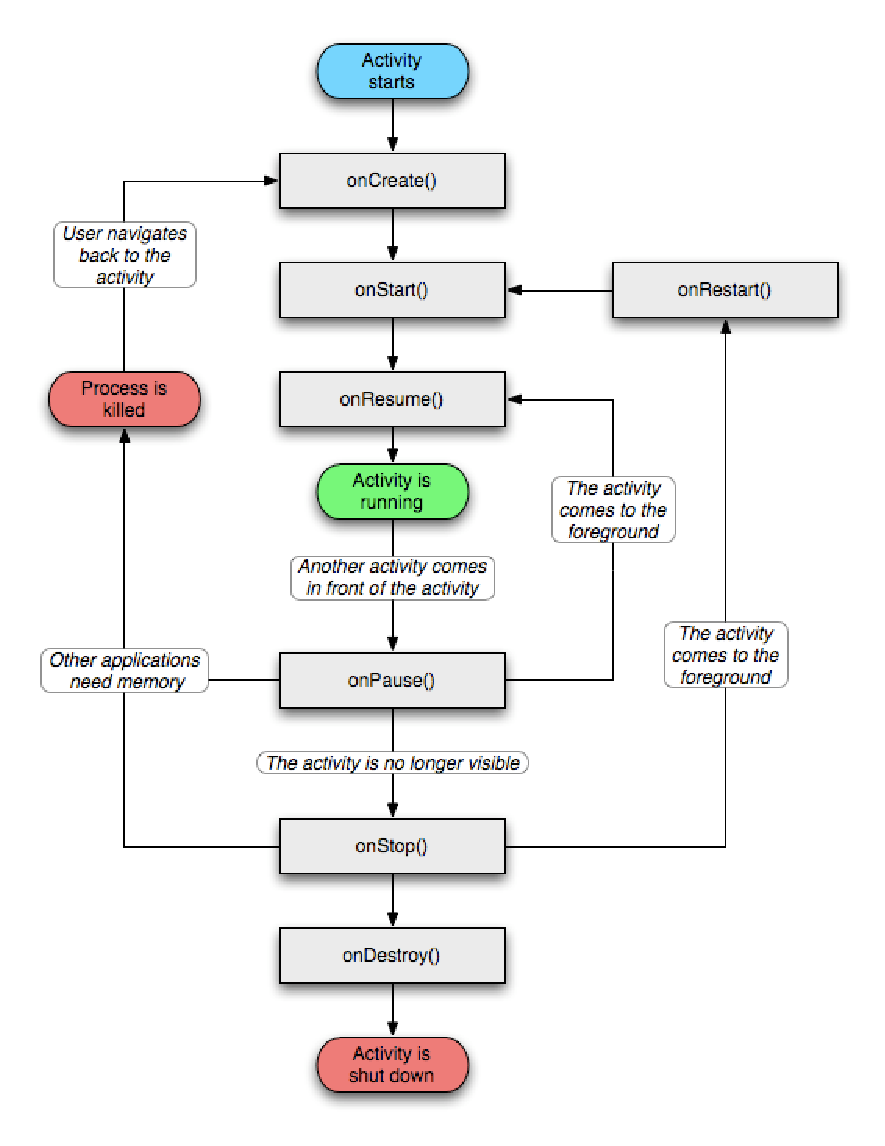
\includegraphics[scale=0.9]{Images/activityLifecycle.eps}
  }
  \caption{Android Activity Life Cycle\protect\footnotemark}
  \end{figure}
  \end{center}
\footnotetext{http://developer.android.com/reference/android/app/Activity.html}
\newpage
 L'affichage de l'activitée \textit{Home} est decris ci-dessous, on peut y
 retrouver une liste personnalisée contenant :
 \begin{itemize}
   \item L'identifiant unique de la caméra.
   \item Suivit de son descriptif.
   \item Puis en indication son l'url.
 \end{itemize}
 On peut également voir en bas de l'image, le menu qui apparait lors de l'appuis
 sur la touche menu du téléphone.\newline
 \begin{center}
    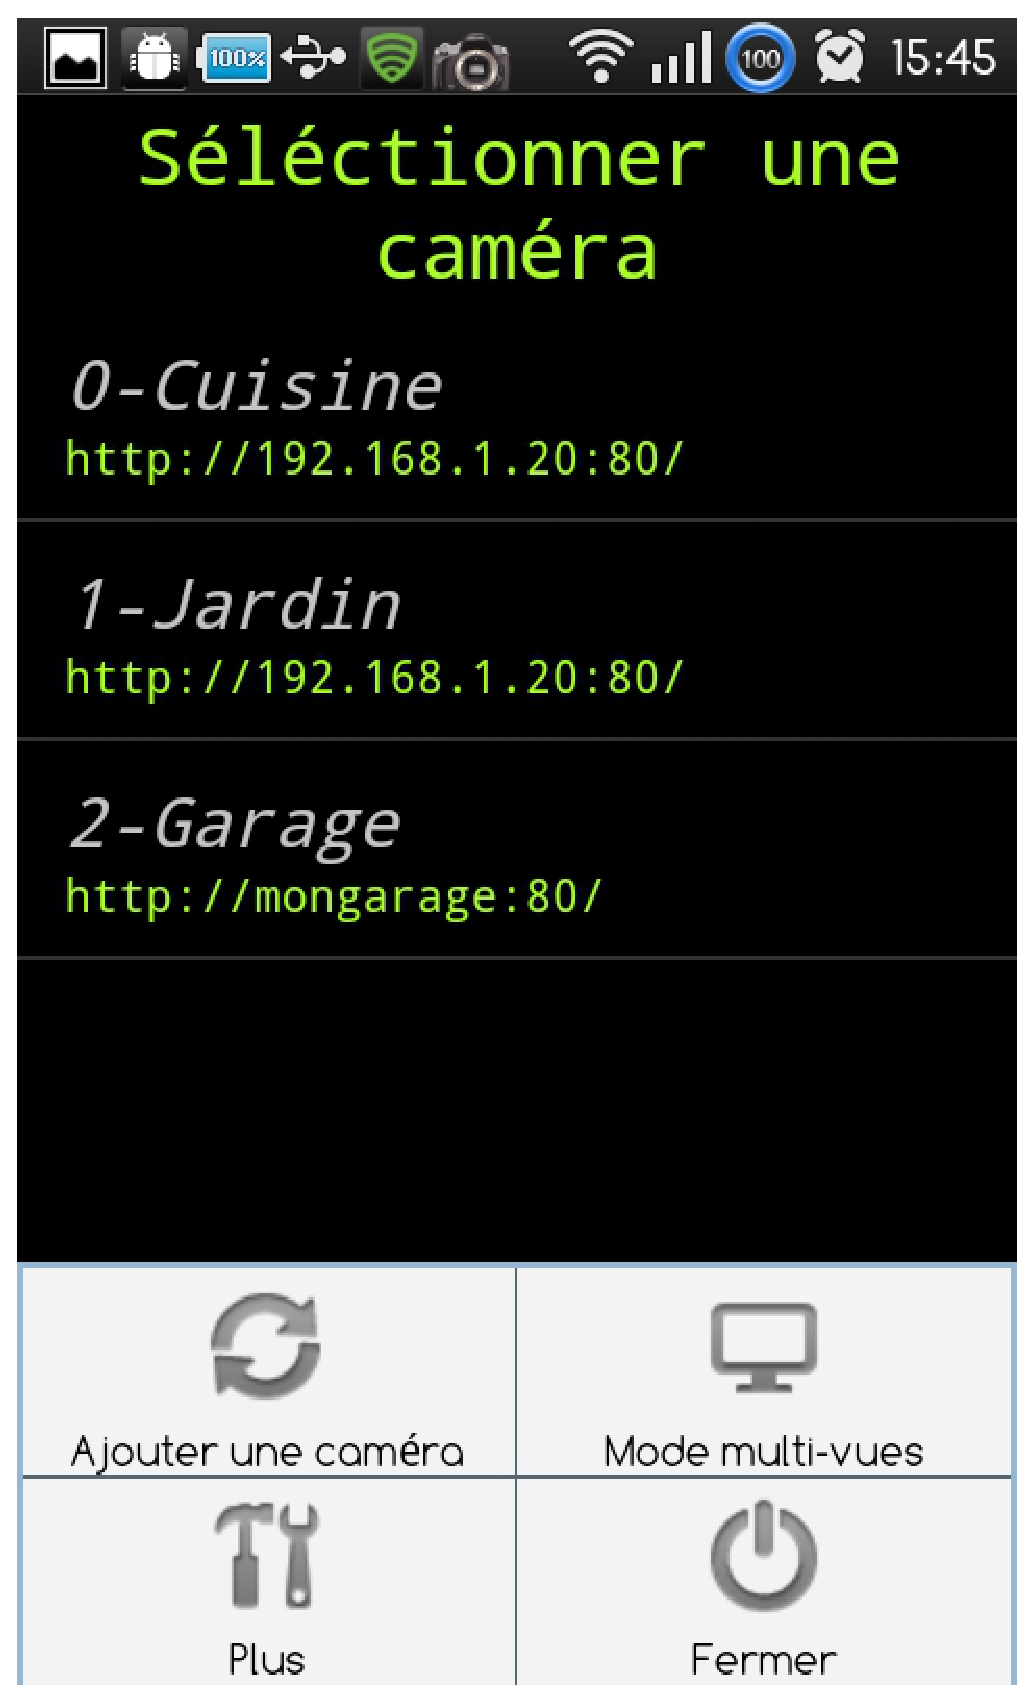
\includegraphics[scale=0.3]{Images/homeScreenShot.eps}
\end{center}

\subsection{Modification et Suppression de l'objet}
Lors d'un appuis long sur une élément de la liste
(\textit{setOnItemLongClickListener}) une alerte apparait pour demander a
l'utilisateur si il souhaite modifier, ou supprimer l'élément (la caméra).
\begin{itemize}
  \item Si il choisit de supprimer l'élément, une seconde alerte apparait pour confirmer
ou annuler son choix. 
\item Si il choisit de modifier la caméra, l'application lance une nouvelle
activité adaptée a la modification de la caméra. Il peut alors appliquer ou
annuler ses changements sur le meme principe que l'ajout d'une caméra.
\end{itemize}
\newpage
\begin{changemargin}{-2cm}{-2cm}
\begin{lstlisting}[caption={Gestion d'un appui long sur un élément de la
liste.}]
public boolean onItemLongClick(AdapterView<?> arg0, 
			View arg1, final int position, long arg3) { 
	AlertDialog alert; 
	AlertDialog.Builder builder = new AlertDialog.Builder(activity);
	builder.setMessage(getString(R.string.messageChoose))
		.setCancelable(false)
		.setPositiveButton(getString(R.string.boutonModifier),
			new DialogInterface.OnClickListener() {
				@Override
				public void onClick(DialogInterface dialog, int id) {
					Intent intent = new Intent(activity.getApplicationContext(),EditCam.class); 
					Bundle objetbunble = new Bundle();
					objetbunble.putSerializable(getString(R.string.camTag),camList.get(position));
					intent.putExtra(getString(R.string.camPosition), position);
					intent.putExtras(objetbunble);
					dialog.cancel();
					startActivityForResult(intent,EDIT_CODE);
		}})
		.setNegativeButton(getString(R.string.boutonSupprimer),
			new DialogInterface.OnClickListener() {
				@Override
				public void onClick(DialogInterface dialog, int id) {
					removeCam(position);
					dialog.cancel();
		}});
		alert = builder.create();
		alert.show();
		return true;
}});
\end{lstlisting}
\end{changemargin}


\section{Communication avec la caméra}


\section{Gestion du flux vidéo}
\subsection{Vue Simple}
Cette partie consiste a décrire l'implémentation de la retransmission de la
video d'une seul sur le téléphone. On trouve cette implémentation dans la classe
\textit{Video.java} qui implémente l'activitée \textit{Video}.
\subsubsection{Cycle de vie}
Précédement nous avons décrit le cycle de vie de l'activitée \textit{Home}.
Ici nous avons également ajouté des fonctionnalité aux differents états afin de
ne pas consomer de ressource inutilement. En effet, lorsque l'activitée n'est
plus au premier plan, il est inutile de continuer a retransmettre le flux
video.\newline
C'est également le cas pour l'utilisation du verrou nous permettant d'empecher
le telephone de se mettre en veille lors de la retransmission de la video. Le
code suivant illustre l'arret de la video et l'utilisation du verrou
(wl).\newline
Il existe plusieurs type de verrou, pour les utiliser il faut recuperer une
instance du gestionnaire d'énérgie \textit{PowerManager} a l'aide de la
fonction : 
\begin{lstlisting}
 PowerManager pm = Context.getSystemService(Context.POWER_SERVICE).
\end{lstlisting}
Puis demander explicitement la création d'un nouveau verrou
(\textit{PowerManager.WakeLock}) a l'aide de la fonction :
\begin{lstlisting}
 pm.newWakeLock(PowerManager.SCREEN_DIM_WAKE_LOCK,"Tag");
\end{lstlisting}
Ces differents verrou sont definit par le premier argument. Il existe quatre
type de verrou dont les caracteristiques sont definie ci-dessous :\newline
\begin{center}
\begin{tabular}{|l|c|c|c|}
\hline
Flag Value & CPU & Screen & Keyboard \\
\hline
PARTIAL\_WAKE\_LOCK & On* & Off & Off \\
SCREEN\_DIM\_WAKE\_LOCK & On & Dim & Off \\ 
SCREEN\_BRIGHT\_WAKE\_LOCK & On & Bright & Off \\
FULL\_WAKE\_LOCK & On & Bright & Bright \\
\hline
\end{tabular}
\newline
\textit{WakeLock flags table\footnote{\label{wakeLockTable}
http://developer.android.com/reference/android/os/PowerManager.html}}
\newline
\end{center}
Nous avons choisi d'utiliser un verrou \textit{SCREEN\_DIM\_WAKE\_LOCK} afin de
garder simplement allumé avec une luminosité au minimum pour ne pas consomer
exessivement la batterie du téléphone.
\newpage
 \begin{lstlisting}[caption={Video
life-cycle}] 
/**
 * Called when Activity start
 */
public void onCreate(Bundle savedInstanceState) {
	super.onCreate(savedInstanceState);
	setContentView(R.layout.video);
	setRequestedOrientation(0);
	
	PowerManager pm = (PowerManager) getSystemService(Context.POWER_SERVICE);
	wl = pm.newWakeLock(PowerManager.SCREEN_DIM_WAKE_LOCK, "My Tags");
	(...)
}
/**
 * Resume video and acquire wakelock when activity resume.
 */
public void onResume() {
	super.onResume();
	wl.acquire();
	if (pause) {
	    mv.resumePlayback();
	    pause = false;
	}
}
 /**
 * Stop video and release wakelock when activity sleep
 */
public void onPause() {
	pause = true;
	wl.release();
	if (mv != null)
	    mv.stopPlayback();
	super.onPause();
}

/**
 * Stop Video before destroy
 */
public void onDestroy() {
	if (mv != null)
	    mv.stopPlayback();
	super.onDestroy();
}
\end{lstlisting}
\subsubsection{ConnectivityManager}
L'accés a internet pour un téléphone disposant d'un systeme d'exploitation
comme Android se fait par des couches phisique de nature differente . Le debit
est donc phortement dependand du support utilisé, c'est pourquoi nous faisons
appel a la classe \textit{ConnectivityManager} afin de récupéré la nature du
support pour definir la resolution aupres de la caméra de la video à envoyer.
Nous avons principalement distingué deux type de réseau : \textit{WiFi} et les
autres réseaux mobile (\textit{3G}, \textit{3G+}, \textit{EDGE}, \ldots).
Afin de definir la correspondance suivant qui nous permet d'obtenir un
taux de raffraichissement correct en \textit{WiFi} (moyenne de 25fps pour une
couverture total) et utilisant la resolution minimal pour les autres reseaux:
\begin{center}
\begin{tabular}{|c|c|}
\hline
Network & Resolution \\
\hline
WiFi &320x240\\
Other &168x120\\
\hline
\end{tabular}
\newline\newline
\end{center}
Pour récupéré le type de réseau on fait une nouvelle fois appel a la
fonction :
\begin{lstlisting}
ConnectivityManager mConnectivity = (ConnectivityManager) getSystemService(Context.CONNECTIVITY_SERVICE);
\end{lstlisting}
Puis en récupérant une instance du réseau actif :
\begin{lstlisting}
NetworkInfo info = mConnectivity.getActiveNetworkInfo();
if (info != null && info.isConnected()) {
  int netType = info.getType();
  if (netType == ConnectivityManager.TYPE_WIFI) {
	/*... Code pour un support de type WiFi ...*/
  } else {
	/*... Code pour les autres supports ...*/
  }
\end{lstlisting}

\subsubsection{Format Vidéo}
Android est capable d'encoder et de decoder un grand nombre de format audio et
video (cf Android Supported Media Formats\footnote{\label{mediaFormat}
http://developer.android.com/guide/appendix/media-formats.html}) a travers
deux protocoles (\textit{HTTP ou RTSP}).\newline
La caméra mise a notre disposition propose uniquement deux formats :
\textit{MJPEG} via le protocol \textit{HTTP} et \textit{MPEG4} via le protocol
\textit{RTSP}.\newline Cependant malgres que le systeme d'exploitation est
capable d'utiliser le protocole \textit{RTSP}, celui-ci ne nous permet pas de
modifier les requetes afin d'y ajouter l'authentification necessaire pour la
lecture de la video. Celle-ci est donc accessible uniquement si la caméra
autorise les utilisateurs anonyme a la visionner.\newline Nous sommes donc
limité au protocol \textit{HTTP} dans lequel nous avons expliqué précédement
la maniere dont nous nous authentifion.\newline\newline
Nous devons donc utiliser le protocol \textit{HTTP} qui fournit une video au
format \textit{MJPEG}. Ce format n'etant pas géré par le
\textit{mediaPlayer}\footnote{\label{mediaPlayer}
http://developer.android.com/reference/android/media/MediaPlayer.html}, nous
avons du trouver un autre moyen d'afficher la video.
\subsubsection{MjpegView}
Grace a la documentation de la caméra\footnote{\label{docAxis}
http://www.axis.com/techsup/cam\_servers/dev/cam\_http\_api\_2.php} on peut
constater que la vidéo est en realité composé de la succession d'une multitude
d'image. Pour afficher la vidéo il faut donc simplement faire defiler chacune
des images recupéré dans la réponse d'une requete de video \textit{MJPEG}.
\newline
Nous avons trouvé sur internet une composant graphique \textit{OpenSource}
appelé \textit{MjpegView}\footnote{\label{MjpegView}
http://www.anddev.org/multimedia-problems-f28/mjpeg-on-android-anyone-t1871-30.html}
réalisant exactement ce traitement.
Nous avons tout de meme du effectuer quelques modifiaction pour l'adapter a
notre utilisation (comme l'ajout d'une fonction \textit{resumePlayback} pour
redemarrer la lecture de la vidéo par exemple).\newline
Comme chacun des composants graphique, il peut etre ajouter dans une activité ou
defini directement dans une vue au format \textit{xml}.\newline
\begin{center}
\begin{lstlisting}[language=XML]
<de.mjpegsample.MjpegView.MjpegView
	android:id="@+id/surfaceView1"
	android:layout_width="fill_parent"
	android:layout_height="fill_parent" />
\end{lstlisting}
 video.xml
\end{center}
\begin{center}
\begin{lstlisting}
public void onCreate(Bundle icicle) {
	super.onCreate(icicle);
	MjpegView mv = new MjpegView(this);
	setContentView(mv);
	mv.setSource(URL);
	mv.setDisplayMode(MjpegView.SIZE_BEST_FIT);
	mv.showFps(true);
}
\end{lstlisting}
mjpegViewer.java
\end{center}





\subsubsection{Interface de controle de la camera}

\subsection{Multi-Vue}
\subsection{Playerthread video}
\subsection{Layout personnalisés et utilisation}

\section{Contrôle de la caméra}

\section{Fonctionnalités avancés}
\subsection{Snapshot}

\subsection{Autres réglage}


\section{Détection de mouvements}
\subsection{Présentation}

\subsection{Utilisation de service Android}


\section{Gestion des préférences}
\subsection{Import / Export}

\subsection{Shared Preferences}

\section{Multilangues, Interface et Partage}

\section{Tests}

\section{Optimisations / Extensions futures}
\subsection{Retransmission du signal audio}
\subsection{Enregistrement vidéo}
\subsection{Edition des fenêtres de détection  de mouvement}
\subsection{Ajout d'evénements suite à la détection (mail / snapshot)}
\subsection{Compte utilisateur}
\clearpage
